\paragraph{QuizziPedia::Front-End::Directives::NewQuestionButtonDirective}

\label{QuizziPedia::Front-End::Directives::NewQuestionButtonDirective}

\begin{figure}[ht]
	\centering
	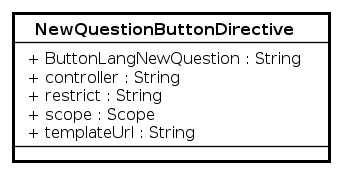
\includegraphics[scale=0.80,keepaspectratio]{UML/Classi/Front-End/QuizziPedia_Front-end_Directives_NewQuestionButtonDirective.png}
	\caption{QuizziPedia::Front-End::Directives::NewQuestionButtonDirective}
\end{figure} 
\FloatBarrier

\begin{itemize}
	\item \textbf{Descrizione}: rappresenta il componente grafico che permette all'utente di posizionarsi nella \textit{view\ped{G}} di creazione di una nuova domanda;
	\item \textbf{Utilizzo}: viene utilizzato per permette all'utente di posizionarsi nella \textit{view\ped{G}} di creazione di una nuova domanda;
	\item \textbf{Relazioni con altre classi}: 
	\begin{itemize}
		\item \textbf{IN \texttt{NewQuestionsButtonsController}}: questa classe permette di effettuare il redirect alla pagina di creazione nuova domanda; 
		\item \textbf{IN \texttt{LangModel}}: rappresenta il modello delle informazioni per la giusta traduzione dell'applicazione;
		\item \textbf{OUT \texttt{QuestionsManagementView}}: \textit{view\ped{G}} contenente l'elenco delle domande create.
	\end{itemize}
	\item \textbf{Attributi}: 
	\begin{itemize}
		\item \texttt{+ ButtonLangNewQuestion: String} \\ Attributo che viene utilizzato per visualizzare la giusta traduzione della \textit{label\ped{G}} per il bottone di creazione di una nuova domanda, in italiano o in inglese;
		\item \texttt{+ controller: String} \\ Stringa contenente il nome del \textit{controller\ped{G}} della direttiva;
		\item \texttt{+ restrict: String} \\ Stringa che permette di definire le modalità di inserimento della direttiva all'interno della pagina;
		\item \texttt{+ scope: Scope} \\ Oggetto scope interno della direttiva, contiene le funzionalità per gestire i dati presenti all'interno;
		\item \texttt{+ templateUrl: String} \\ Stringa contenente il percorso del file \textit{HTML\ped{G}} che contiene la direttive.
	\end{itemize}
\end{itemize}